\documentclass[11pt]{article}

\usepackage{graphicx}
\usepackage[margin=1in]{geometry}
\usepackage[dvipsnames]{xcolor}
\usepackage[most]{tcolorbox}
\usepackage[colorlinks=true, linkcolor=blue]{hyperref}
\usepackage{subcaption, float}

\newtcolorbox{definition}[1][]{
  colback=blue!5!white,
  colframe=blue!75!black,
  fonttitle=\bfseries,
  title=Definition: #1
}

\newtcolorbox{warning}{
  colback=red!5!white,
  colframe=red!75!black,
  fonttitle=\bfseries,
  title=Warning
}

\newtcolorbox{note}[1][]{
  colback=green!5!white,
  colframe=green!75!black,
  fonttitle=\bfseries,
  title=#1
}

\newtcolorbox{note_special}[1][]{
  colback=orange!5!white,
  colframe=orange!75!black,
  fonttitle=\bfseries,
  title=#1,
  breakable
}

\begin{document}


\begin{titlepage}
    \centering
    
    
\includegraphics[width=0.4\textwidth]{UCT-logo.png}\\[2cm] 
    
    \textsc{\LARGE University of Cape Town}\\[1.5cm]
    
    \rule{\linewidth}{0.5mm} \\[0.4cm]
    { \huge \bfseries CSC2042S: Machine Learning \\[0.4cm] }
    \rule{\linewidth}{0.5mm} \\[1.5cm]
    
    { \Large Author: George Goodey }
    
    \vfill

    {\large \today}
    
\end{titlepage}

\tableofcontents
\newpage

% Here is some standard text for my notes. 

% \begin{definition}[Thermodynamics]
% The branch of physics that deals with the relationships between heat and other forms of energy.
% \end{definition}

% \begin{warning}
% Do not confuse heat with temperature! 
% \end{warning}

\section{Supervised learning}

\subsection{What is machine learning?}
\begin{definition}[Machine Learning]
Machine learning is the study of algorithms that:
\begin{itemize}
    \item improve their performance $P$ (according to a criterion that measures success)
    \item at some task $T$
    \item with experience $E$ (from data examples).
\end{itemize}
\end{definition}
$\quad$\\[0em]
A well-defined task is given by $<P,T,E>$. For example:
\begin{itemize}
    \item \textbf{Image classification:} $<$Accuracy, Classify handwritten digits, Dataset of labelled images$>$.
    \item \textbf{Chess:} $<$Playing quality, Play chess against human, Dataset of old games$>$.
    \item \textbf{ChatGPT:} $<$Quality of conversation, Generate responses, All text on the web$>$.
\end{itemize}

\subsection{Types of machine learning}
There are many types:
\begin{itemize}
    \item Supervised learning.
    \item Unsupervised learning.
    \item Reinforcement learning.
    \item etc.
\end{itemize}

\subsubsection{Unsupervised learning}
The problem is framed as finding structure in $x$ without labels (no $y$). Inputs are examples in the dataset represented by \textit{features}. Data $D$ is $|D|$ examples $\{x_1,x_2,\dots,x_{|D|}\}$ without any labels. Given a new example $x$, where does this fit into the data? 


\subsection{Simple linear regression}
A simple linear regression model predicts the output as a linear function of one input feature $x$: $y=wx+b$, otherwise known as a straight line function. Changes in $x$ imply a proportional change in $y$. Even if the relationship is not perfectly linear, linear regression can still be effective as an approximation or baseline model.
\begin{figure}[H]
    \centering
    \begin{subfigure}{0.8\textwidth}
        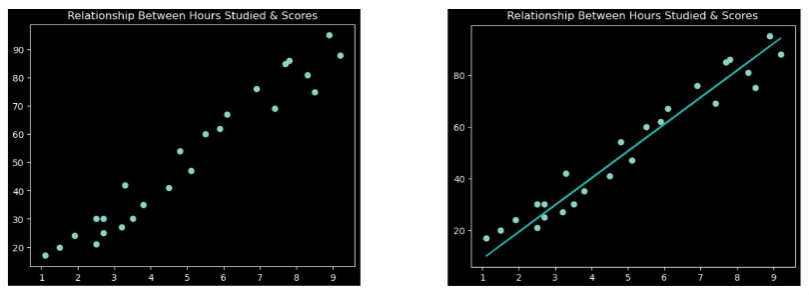
\includegraphics[width=\linewidth]{Pictures/SLR_1.png}
    \end{subfigure}
\end{figure}

\subsubsection{Loss function}
For each input, linear regression produces an estimate $\hat{y}_i=w\cdot x_i+b$. We want to set $w$ and $b$ to minimize the distance between our estimate $\hat{y}_i$ (prediction) and the true $y_i$. We want to minimize this distance/error across our entire training set $\{(x_1,y_1),(x_2,y_2),\dots,(x_N,y_N)\}$.
\\[1em]
A principled way to define the learning problem is with a loss function (also known as a cost function): $L(\hat{y}_i,y_i)$ measuring how close the model prediction $\hat{y}_i$ is to the observed data $y_i$. If the model fits the data well, so that $y_i\approx \hat{y}_i$, then the loss function should take a small value, and vice versa. For this, we can use the squared error loss.
\begin{figure}[H]
    \centering
    \begin{subfigure}{0.5\textwidth}
        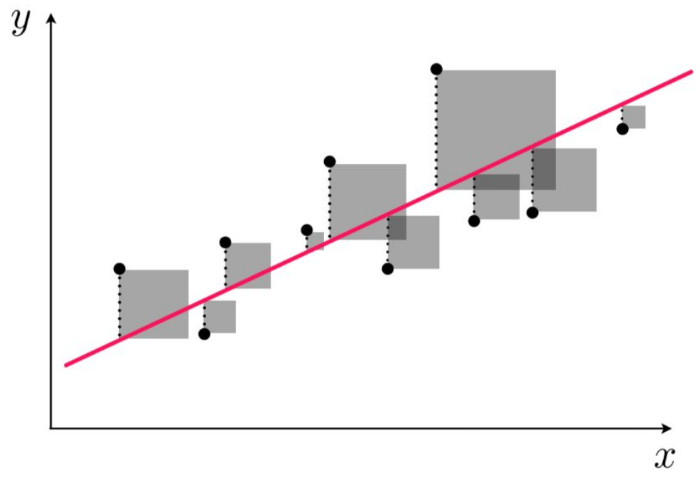
\includegraphics[width=\linewidth]{Pictures/SLR_2.png}
    \end{subfigure}
\end{figure}
$\quad$\\[-1em]
The squared error loss measures how good your linear regression model with parameters $w,b$ fits the data. For a single data point $(x_i,y_i)$:
\begin{align*}
    L(\hat{y}_i,y_i)&=(y_i-\hat{y}_i)^2 \\
    &=(y_i-f(x_i;w,b))^2 \\
    &=(y_i-(w\cdot x+b))^2 \\
    &=(y_i-w\cdot x-b)^2
\end{align*}
We want to find the weight that minimizes the loss, averaged over all examples in our training set.
$$
\boxed{J(w,b)=\frac{1}{N}\sum_{i=1}^{N}L(\hat{y}_i,y_i)}
$$
\begin{note}[Note: Why as a function of $w$ and $b$?]
These are the variables we want to learn!
\end{note}
$\quad$\\[-1em]
All examples $(x_i,y_i)$ in the function are determined by whatever is in the training set. This is out of our control. Now, we want to find:
$$
\hat{w},\hat{b}=\underset{w,b}{\text{argmin}}J(w,b)
$$
For linear regression, the loss function (mean squared error) is convex. This means it has a single global minimum and no local minima. Linear regression has a closed form solution. The question is, how do we find $\hat{w},\hat{b}=\underset{w,b}{\text{argmin}}J(w,b)$?
\begin{enumerate}
    \item Take the partial derivative of $J$ with respect to $w$ and $b$.
    \item Set the partial derivative equal to 0.
    \item Solve for $w$ and $b$.
\end{enumerate}
\begin{note_special}[Derivation]
\textbf{Derivation w.r.t $b$:}
\begin{align*}
    \frac{\partial}{\partial b}J(w,b)&=\frac{\partial}{\partial b}\frac{1}{N}\sum_{i=1}^{N}(y_i-wx_i-b)^2 \\
    &=\frac{-2}{N}\sum_{i=1}^{N}(y_i-wx_i-b) \\
    0&=\sum_{i=1}^N(y_i-wx_i-b) \quad\text{(Setting equal to 0)} \\
    0&=\sum_{i=1}^{N}y_i -w\sum_{i=1}^{N}x_i-Nb \\
    \hat{b}&=\bar{y}-\hat{w}\bar{x}
\end{align*}
\textbf{Derivation w.r.t $w$:}\\
Before differentiating w.r.t $w$, substitute this expression for $b$ back into the cost so that $J$ becomes a function of $w$ only:
$$
J(w)=\frac{1}{N}\sum_{i=1}^{N}\Big[y_i-wx_i-(\bar{y}-w\bar{x})\Big]^2=\frac{1}{N}\sum_{i=1}^{N}\Big[(y_i-\bar{y})-w(x_i-\bar{x})\Big]^2
$$
Now differentiate w.r.t $w$:
$$
\frac{d}{dw}J(w)=\frac{-2}{N}\sum_{i=1}^{N}\big[(y_i-\bar{y})-w(x_i-\bar{x})\big]\big[(x_i-\bar{x})\big]
$$
Set the derivative to 0 and simplify:
\begin{align*}
    0&=\frac{-2}{N}\Big[\sum_{i=1}^{N}(y_i-\bar{y})(x_i-\bar{x})-w\sum_{i=1}^{N}(x_i-\bar{x})^2\Big] \\
    w\sum_{i=1}^{N}(x_i-\bar{x})^2&=\sum_{i=1}^{N}(y_i-\bar{y})(x_i-\bar{x}) \\
    \hat{w}&=\frac{\sum_{i=1}^{N}(y_i-\bar{y})(x_i-\bar{x})}{\sum_{i=1}^{N}(x_i-\bar{x})^2}
\end{align*}
\end{note_special}

\subsection{Logistic regression}
\subsubsection{Probability basics}
\begin{itemize}
    \item $P(A)$: probability of event $A$.
    \item $P(A^c)$: probability of event $A$ not happening.
    \item $P(A|B)$: probability of $A$ given $B$ (conditional probability).
    \item For any event $A$, $0\leq P(A)\leq 1$.
    \item Let $S$ be the sample space of all possible events, then $P(S)=1$.
    \item For any event $A$, $P(A^c)=1-P(A)\iff P(A)=1-P(A^c)$.
\end{itemize}

\subsubsection{Discriminative classifier}
Discriminative models learn boundaries between classes. For example, suppose we are classifying cat vs. dog images. The input $x$ is the image (matrix of pixel values). The output $y$ is the class (either cat or dog).
The goal of classification is to find the correct class $y$ given input $x$. To classify, we compute: $y=\underset{y\in C}{\text{argmax}}P(y|x)$.

\subsubsection{Logistic regression}
We introduce the sigmoid function:
$$
\sigma(z)=\frac{1}{1+e^{-z}}
$$
\begin{figure}[H]
    \centering
    \begin{subfigure}{0.5\textwidth}
        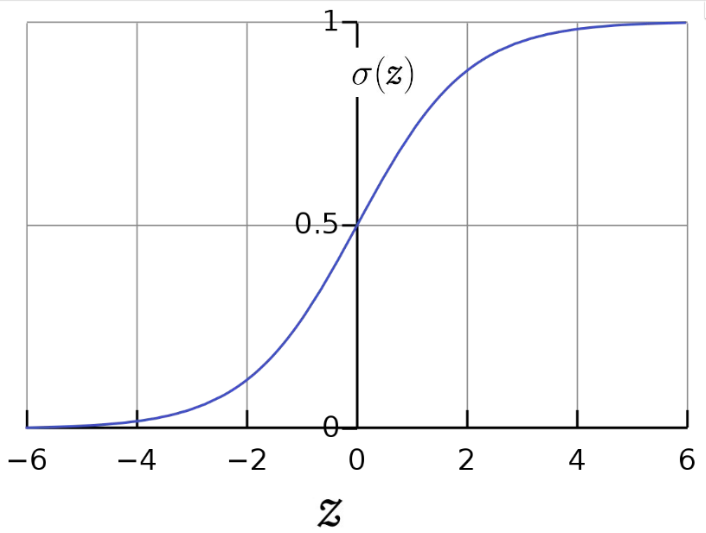
\includegraphics[width=\linewidth]{Pictures/LR_1.png}
    \end{subfigure}
\end{figure}
$\quad$\\[-1em]
The sigmoid function is called a logistic function. It squeezes any input value between 0 and 1. To classify the input $\mathbf{x}$:
\begin{itemize}
    \item Compute the weighted sum, $z=\sum w_ix_i+b=\mathbf{w}\cdot\mathbf{x}+b$.
    \item Pass $z$ through the sigmoid function, $\sigma(\mathbf{w}\cdot\mathbf{x}+b)$.
    \item Treat the result as a probability. $$ P(y=1|\mathbf{x})=\sigma(\mathbf{w}\cdot\mathbf{x}+b)=\frac{1}{1+\text{exp}(-\mathbf{w}\cdot\mathbf{x}-b)} $$
\end{itemize}
A key property of the sigmoid function: $1-\sigma(z)=\sigma(-z)$.
\begin{note_special}[Derivation]
\begin{align*}
    P(y=0|\mathbf{x})&=1-\sigma(\mathbf{w}\cdot\mathbf{x}+b) \\
    &=1-\frac{1}{1+\text{exp}(-\mathbf{w}\cdot\mathbf{x}-b)} \\
    &=\frac{\text{exp}(-\mathbf{w}\cdot\mathbf{x}-b)}{1+\text{exp}(-\mathbf{w}\cdot\mathbf{x}-b)}\times\frac{\text{exp}(\mathbf{w}\cdot\mathbf{x}+b)}{\text{exp}(\mathbf{w}\cdot\mathbf{x}+b)} \\
    &=\frac{1}{1+\text{exp}(\mathbf{w}\cdot\mathbf{x}+b)} \\
    &=\sigma(-\mathbf{w}\cdot\mathbf{x}-b)
\end{align*}
\end{note_special}
$\quad$\\[-1em]
Now, we have a way to compute both $P(y=1|\mathbf{x})$ and $P(y=0|\mathbf{x})$. We can now make decisions:
$$
\text{decision}(\mathbf{x})=\begin{cases}
    1 & \text{if }P(y=1|\mathbf{x})>0.5 \\
    0 & \text{otherwise}
\end{cases}
$$
The decision boundary of $P(y|x)=0.5$ is defined where $\mathbf{w}\cdot\mathbf{x}+b=0$. This is the default decision boundary in logistic regression. However, you can specify a different decision boundary to suit your task.
\begin{itemize}
    \item Choose a higher value, like $P(y=1|\mathbf{x})>0.9$, if you want the model to be confident before flagging an instance of a positive class.
    \item Choose a lower value, like $P(y=1|\mathbf{x})>0.2$, if you don't want to risk missing instances of the positive cass (e.g. medical diagnosis).
\end{itemize}

\subsubsection{Example}
Predict if a fire weather warning should be announced.
\begin{itemize}
    \item $x_1$: temperature in $C^\circ$.
    \item $x_2$: wind speed in km/h.
    \item $y=0$: no warning needed.
    \item $y=1$: warning needed.
\end{itemize}
Suppose the weights are $\mathbf{w}=[0.1,0.05]$ and the bias term is $b=-5$. For an input vector $\mathbf{x}=[25,60]$,
\begin{align*}
    P(y=1|\mathbf{x})&=\sigma(\mathbf{w}\cdot\mathbf{x}+b)=\sigma((0.1)(25)+(0.05)(60)-5)=\sigma(0.5)=0.622 \\
    P(y=0|\mathbf{x})&=1-P(y=1|\mathbf{x})=1-0.622=0.378
\end{align*}
Since $P(y=1|\mathbf{x})=0.622>0.5$, a warning should be given.

\subsection{Cross-entropy loss}
\subsubsection{Log probabilities}
\begin{definition}[Log probability]
    A log probability is a logarithm of a probability value, $\log P(X)$. This represents probabilities on a logarithmic scale $(-\infty,0]$ instead of the usual $[0,1]$ probability interval.
\end{definition}
$\quad$\\[-1em]
A useful property of log properties:
$$
\log P(ABC)=\log(P(A)\times P(B)\times P(C))=\log P(A)+\log P(B)+\log P(C)
$$

\subsubsection{Loss function}
We use conditional \textbf{maximum likelihood estimation}:
\begin{itemize}
    \item Find parameters that \textbf{maximize the probability of the true labels} in the training data given the observations.
    \item For binary classification, since there are 2 discrete outcomes, we can express the classifier's probability of the true label $y$ as:
$$
P(y|\mathbf{x})=\hat{y}^y(1-\hat{y})^{1-y}
$$
    \item If $y=1$, this simplifies to $\hat{y}$ which is $P(y=1|\mathbf{x})$.
    \item If $y=0$, this simplifies to $1-\hat{y}$ which is $P(y=0|\mathbf{x})$.
\end{itemize}
$\quad$\\[-1em]
We can rewrite this in terms of log probabilities:
\begin{align*}
    \log P(y|\mathbf{x})&=\log\big[\hat{y}^y(1-\hat{y}^{1-y})\big] \\
    &=y\log\hat{y}+(1-y)\log(1-\hat{y})
\end{align*}
We can then turn this into a loss function to be minimized by using the negative log likelihood. This is called the \textbf{cross-entropy loss} between the prediction and the true class.
\begin{align*}
    L_{\text{CE}}(\hat{y},y)&=-\log P(y|\mathbf{x}) \\
    &=-\big[y\log\hat{y}+(1-y)\log(1-\hat{y})\big] \\
    &=-\big[y\log[\sigma(\mathbf{w}\cdot\mathbf{x}+b)]+(1-y)\log[\sigma(-\mathbf{w}\cdot\mathbf{x}-b)]\big]
\end{align*}
By minimizing this loss, we maximize the probabilities assigned to the true labels by the logistic regression model.

\subsubsection{Example}
Predict if a fire weather warning should be announced.
\begin{itemize}
    \item $x_1$: temperature in $C^\circ$.
    \item $x_2$: wind speed in km/h.
    \item $y=0$: no warning needed.
    \item $y=1$: warning needed.
\end{itemize}
Suppose the weights are $\mathbf{w}=[0.1,0.05]$ and the bias term is $b=-5$. \\\\ 
For an input vector $\mathbf{x}=[25,60]$ and true label $y=1$:
\begin{flalign*}
    P(y=1|\mathbf{x})&=\sigma(\mathbf{w}\cdot\mathbf{x}+b)=0.622 &\\
    L_{\text{CE}}(\hat{y},{y})&=-\log P(y=1|\mathbf{x})=-\log 0.622 = 0.206 &
\end{flalign*}
For an input vector $\mathbf{x}=[25,60]$ and true label $y=0$:
\begin{flalign*}
    P(y=0|\mathbf{x})&=1-\sigma(\mathbf{w}\cdot\mathbf{x}+b)=0.378 &\\
    L_{\text{CE}}(\hat{y},y)&=-\log P(y=0|\mathbf{x})=-\log 0.378=0.423 &
\end{flalign*}
Since the loss of true label $y=1$ is lower, we should give a warning.
\begin{note}[Note]
The loss is higher if the model is wrong. Lower probabilities assigned to the true class implies a higher loss.
\end{note}

\subsubsection{Objective function}
Given the cross-entropy loss, we want to minimize this loss on average across our training set:
$$
\boxed{\frac{1}{N}\sum_{i=1}^{N}L_{\text{CE}}(\hat{y}_i,y_i)}
$$
If we can adjust parameters $\mathbf{w}$ and $b$ to lower the loss over all instances in the training set, we will have a good classifier. This is the essence of modern machine learning and deep learning.

\subsubsection{Optimization}
Let the loss function be parameterized by parameters $\theta=(\mathbf{w},b)$. We represent $\hat{y}$ as $f(\mathbf{x};\theta)$. We want to find parameters that minimize the loss averaged over all examples in our training set.
$$
\hat{\theta}=\underset{\theta}{\text{argmin}}\hspace{2pt}\frac{1}{N}\sum_{i=1}^{N}L_{\text{CE}}(f(\mathbf{x};\theta),y_i)
$$ 
There is \textbf{no closed form solution} for finding minimizing weights for logistic regression. Instead, we will use an iterative method called gradient descent.

\subsection{Gradient descent}
\begin{definition}[Gradient descent]
Gradient descent is an optimization algorithm that iteratively updates parameters by moving in the opposite direction of the gradient of the loss function, in order to minimize the loss.
\end{definition}
\subsubsection{Loss function}
We want parameters $\mathbf{w},b$ that minimize loss averaged over $m$ examples in our training set. We denote the average loss as $J(\mathbf{w},b)$ with $\hat{y}_i=f(\mathbf{x}_i;\mathbf{w},b)$ written as a function of inputs and parameters.
$$
J(\mathbf{w},b)=\frac{1}{m}\sum_{i=1}^{m}\big[y_i\log\sigma(\mathbf{w}\cdot\mathbf{x}_i+b)+(1-y_i)\log[1-\sigma(\mathbf{w}\cdot\mathbf{x}_i+b)]\big]
$$
Now, we want to find:
$$
\hat{\mathbf{w}},\hat{b}=\underset{\mathbf{w},b}{\text{argmin}}\hspace{2pt}J(\mathbf{w},b)
$$

\subsubsection{Optimization}
For logistic regression, the loss function is convex. Gradient descent from any point is guarenteed to find the minimum. Here is a visualization for a single scalar $w$: Given the current $w$, move in the reverse direction from the function slope.
\begin{figure}[H]
    \centering
    \begin{subfigure}{\textwidth}
        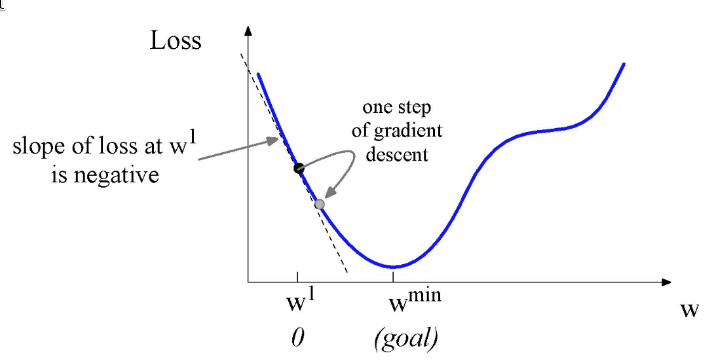
\includegraphics[width=\linewidth]{Pictures/GD_1.png}
    \end{subfigure}
\end{figure}
$\quad$\\[-1em]
The loss is a function of multiple parameters $w_1,\dots,w_n,b$:
$$
L_{\text{CE}}=-\big[y\log\sigma(\mathbf{w}\cdot\mathbf{x}+b)+(1-y)\log[1-\sigma(\mathbf{w}\cdot\mathbf{x}+b)]\big]
$$
The gradient of this loss with respect to the parameters $\theta$ will be a vector of partial derivatives.
$$
\nabla_{\theta}L=\frac{\partial L}{\partial \theta}=\begin{bmatrix}
    \frac{\partial L}{\partial w_1} \\
    \frac{\partial L}{\partial w_2} \\
    \vdots \\
    \frac{\partial L}{\partial w_n} \\
    \frac{\partial L}{\partial b}
\end{bmatrix}
$$
For models with $n$-dimensional weight vectors:
\begin{itemize}
    \item For each dimension $w_i$, the gradient component $i$ tells us the slope w.r.t that parameter.
    \item We express the slope as the partial derivative of $L$ w.r.t $w_i$.
    \item The gradient is defined as the vector of these partial derivatives.
\end{itemize}

\subsubsection{Learning rate}
$$
\mathbf{w}^{t+1}=\mathbf{w}^t-\eta\frac{d}{dw}L(f(\mathbf{x};\mathbf{w}),y)
$$
The gradient tells us:
\begin{itemize}
    \item \textbf{Sign:} which way to move (left, right, up, down).
    \item \textbf{Magnitude:} how steep/big the update is.
\end{itemize}
To control the step size, the value of the gradient is weighted by a learning rate $\eta$. A higher value of $\eta$ means $\mathbf{w}$ changes faster. This is considered a hyperparameter.
\begin{itemize}
    \item If the learning rate is too high, it will take big steps and overshoot.
    \item If the learning rate is too low, it will take too long to converge.
\end{itemize}

\subsubsection{Optimization (continued)}
How do we find $\hat{\theta}=\underset{\theta}{\text{argmin}}\hspace{2pt}\frac{1}{m}\sum_{i=1}^{m}L_{\text{CE}}(f(\mathbf{x};\theta), y_i)$? We do the following iteratively:
\begin{itemize}
    \item Compute the derivative of the loss function with respect to the parameters.
    \item Update the parameters to move in the opposite direction of the gradient.
\end{itemize}
The partial derivatives for logistic regression:
$$
\boxed{\frac{\partial L}{\partial w_i}=[\sigma(\mathbf{w}\cdot\mathbf{x}+b)-y]x_i}\quad\quad\boxed{\frac{\partial L}{\partial b}=\sigma(\mathbf{w}\cdot\mathbf{x}+b)-y}
$$

\subsubsection{Gradient descent formula}
The final question for updating parameters $\theta$ based on the gradient is:
$$
\theta^{t+1}=\theta^t-\eta\nabla_{\theta}L(f(\mathbf{x};\theta),y)
$$
\begin{note}[Note]
Gradient descent can be applied to any model with any number of parameters. Gradient descent is a general optimization method, not just for logistic regression!
\end{note}

\subsection{Stochastic gradient descent}
\begin{definition}[Stochastic gradient descent]
Stochastic gradient descent (SGD) iteratively updates parameters. It approximates the true gradient by using a subset of data at each step.
\end{definition}
$\quad$\\[-1em]
At each step, a random subset of examples is sampled. Both the gradient is computed and the parameters are updated based on this subset.
$$
\theta^{t+1}=\theta^{t}-\eta\frac{1}{B}\sum_{i=1}^{B}\nabla_{\theta}L(f(\mathbf{x}_i;\theta), y_i)
$$
\textbf{Batch / mini-batch:} The subset of data used for SGD at a particular training step. \\
\textbf{Batch size:} The number of training examples in each batch. \textbf{This is a hyperparameter.}
\subsubsection{Batching}
In practice, it's computationally expensive to apply gradient descent to the entire training set simultaneously. This is due to the high computational/memory requirements for large datasets and the slow convergence. Instead, we employ the principle of batching. \\\\
Traverse the training set in batches, $B$ examples at a time, updating parameters based on gradient w.r.t average loss of the batch.
$$
J_B(\theta)=\frac{1}{B}\sum_{i=1}^{B}L(f(\mathbf{x}_i;\theta), y_i)
$$
The gradient of the cross-entropy loss averaged over all $B$ examples in a batch is the average of the individual sample gradients.
$$
\nabla_{\theta}J_B(\theta)=\frac{1}{B}\sum_{i=1}^{B}\nabla_{\theta}L(f(\mathbf{x}_i;\theta), y_i)
$$

\subsubsection{Example}
Assume initial parameters $\theta^0$ are all zero: $w_1=w_2=b=0$. let's perform a SGD update based on one example in the training set. Let $\mathbf{x}=[3,2]$ with label $y=1$. Then,
\begin{align*}
    \nabla_{\theta}=\begin{bmatrix}
        \frac{\partial L}{\partial w_1} \\
        \frac{\partial L}{\partial w_2} \\
        \frac{\partial L}{\partial b}
    \end{bmatrix}
    &=\begin{bmatrix}
        [\sigma(\mathbf{w}\cdot\mathbf{x}+b)-y]x_1 \\
        [\sigma(\mathbf{w}\cdot\mathbf{x}+b)-y]x_2 \\
        [\sigma(\mathbf{w}\cdot\mathbf{x}+b)-y]
    \end{bmatrix} \\
    &=\begin{bmatrix}
        [\sigma(0)-1](3) \\
        [\sigma(0)-1](2) \\
        [\sigma(0)-1]
    \end{bmatrix} \\
    &=\begin{bmatrix}
        -1.5 \\
        -1.0 \\
        -0.5
    \end{bmatrix}
\end{align*}
Now that we have the gradient vector, we compute the new parameter values with gradient descent. Set the learning rate $\eta=0.1$.
\begin{align*}
    \theta^1&=\theta^0-\eta\nabla_\theta L \\
    &=\begin{bmatrix}
        0 \\
        0 \\
        0
    \end{bmatrix}
    -(0.1)\begin{bmatrix}
        -1.5 \\
        -1.0 \\
        -0.5
    \end{bmatrix} \\
    &=\begin{bmatrix}
        -0.15 \\
        -0.10 \\
        -0.05
    \end{bmatrix}
\end{align*}

\subsubsection{Vectorization}
Construct matrices and vectors that allow us to process a batch as a matrix/vector computation.
Let the rows of matrix $X$ represent input features of individual trainign samples with $B$ examples in the batch and $n$ input features:
$$
X=\begin{bmatrix}
    x_{11} & x_{12} & \cdots & x_{1n} \\
    x_{21} & x_{22} & \cdots & x_{2n} \\
    \vdots & \vdots & \ddots & \vdots \\
    x_{B1} & x_{B2} & \cdots & x_{Bn}
\end{bmatrix}_{B\times n}
$$
The vector $\mathbf{w}$ is the weight parameters. Let $\mathbf{b}$ be a $B$-dimensional vector repeating bias parameter $b$.
$$
\mathbf{w}=\begin{bmatrix}
    w_1 \\
    w_2 \\
    \vdots \\
    w_n 
\end{bmatrix}_{n\times 1}
\quad\quad
\mathbf{b}=\begin{bmatrix}
    b \\
    b \\
    \vdots \\
    b
\end{bmatrix}_{B\times 1}
$$
Then we can compute the weighted sums $\mathbf{w}\cdot\mathbf{x}_i+b$ simultaneously for all $B$ examples with matrix multiplication.
$$
X\mathbf{w}+\mathbf{b}=\begin{bmatrix}
    w_1x_{11}+w_2x_{12}+\cdots+w_nx_{1n}+b \\
    w_1x_{21}+w_2x_{22}+\cdots+w_nx_{2n}+b \\
    \vdots \\
    w_1x_{B1}+w_2x_{B2}+\cdots+w_nx_{Bn}+b
\end{bmatrix}_{B\times 1}
$$
If we aply the sigmoid function to each element of this vector:
$$
\hat{\mathbf{y}}=\sigma(X\mathbf{w}+\mathbf{b})=\begin{bmatrix}
    \sigma(w_1x_{11}+w_2x_{12}+\cdots+w_nx_{1n}+b) \\
    \sigma(w_1x_{21}+w_2x_{22}+\cdots+w_nx_{2n}+b) \\
    \vdots \\
    \sigma(w_1x_{B1}+w_2x_{B2}+\cdots+w_nx_{Bn}+b)
\end{bmatrix}_{B\times 1}
=\begin{bmatrix}
    \hat{y}_1 \\
    \hat{y}_2 \\
    \vdots \\
    \hat{y}_B
\end{bmatrix}
$$
\end{document}